\chapter{Marco Te\'orico}

\section{Internet de las Cosas (IoT) en el Ámbito Industrial}

\par El \textbf{Internet Industrial de las Cosas (IIoT)} representa la convergencia de las tecnologías de la información (IT) y las tecnologías operativas (OT), posicionándose como el motor fundamental de la \textbf{Cuarta Revolución Industrial} \cite{WEF_IIoT_2018}. A diferencia del IoT orientado al consumidor, el IIoT se define como la aplicación de estas tecnologías en entornos industriales o empresariales para crear valor a través de procesos, cadenas de suministro, productos y servicios inteligentes \cite{Connected_Everything_2016}. Esta evolución trasciende la interconexión de objetos cotidianos para enfocarse en la red de equipos, máquinas, computadoras y personas, permitiendo operaciones industriales inteligentes mediante el uso de análisis de datos avanzados.\\

\par La complejidad inherente del IIoT radica en que sus soluciones no operan de forma aislada, sino que se integran en sistemas operativos de gran escala, creando interdependencias críticas entre sus componentes. Para comprender su funcionamiento, la literatura científica suele estructurar el ecosistema en tres niveles fundamentales (ver figura \ref{fig:imagen1}) \cite{Salazar_IoT_2014}. En el ámbito nacional, antecedentes recientes han demostrado la viabilidad de arquitecturas de monitoreo en tiempo real en el contexto universitario \cite{Garrido_Tesis_2025}.

\begin{figure} [htbp]
    \centering
    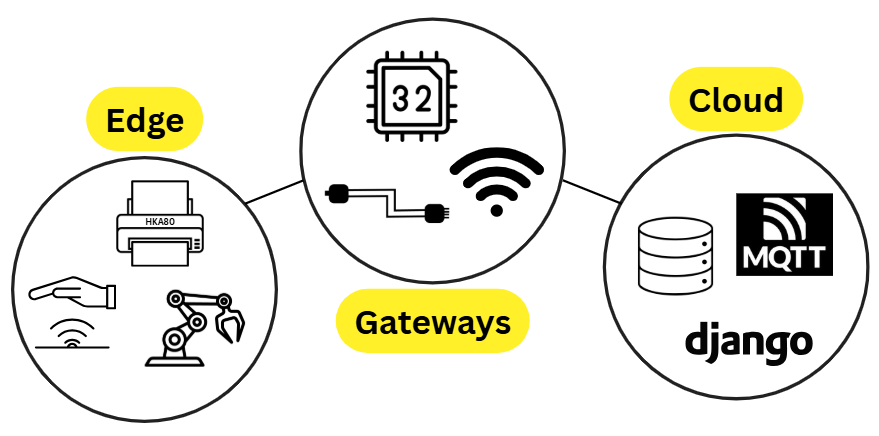
\includegraphics[width=0.8\linewidth]{Img/iiot_diagram.png}
    \caption{Diagrama de los tres niveles fundamentales en un sistema IIoT.}
    \label{fig:imagen1}
\end{figure}

\begin{enumerate}
    \item \textbf{Funcionalidad de borde (Edge):} Sensores y actuadores conectados físicamente a equipos y materiales.
    \item \textbf{Pasarelas de datos (Gateways):} Mecanismos encargados de la recepción y transmisión transparente de información entre los dispositivos de borde y los servidores en red.
    \item \textbf{Gestión y análisis de datos:} Sistemas basados habitualmente en la nube para la recopilación, enlace y análisis de la información para la toma de decisiones.
\end{enumerate}

\par Un pilar en esta arquitectura es la transformación de equipos convencionles en \textbf{productos inteligentes}. Según la Universidad de Cambridge, un activo físico integrado en IIoT posee identidad única \cite{Connected_Everything_2016}, capacidad de comunicación efectiva con su entorno, almacenamiento de datos propio y autonomía para participar en decisiones relevantes para su funcionamiento. Esta metamorfosis de sistemas previamente aislados hacia una red conectada permite recolectar datos \say{no productivos} (como diagnóticos de mantenimiento o estados operativos) que antes eran inaccesibles, optimizando así el ciclo de vida del producto y la eficiencia general del ecosistema industrial.\\

\par Finalmente, la transición de equipos aislados a sistemas hiperconectados introduce una superficie de ataque significativamente mayor, donde la seguridad deja de ser una característica opcional para convertirse en un requisito de diseño mandatorio. El World Economic Forum advierte que el estado de vulnerabilidad en el sector industrial es insostenible sin la adopción de protocolos de seguridad y protección activa \cite{WEF_IIoT_2018}. En el contexto fiscal, donde la integridad de los datos es innegociable, el ecosistema IIoT requiere mecanismos de \say{endurecimiento activo} (active hardening) que garanticen la tríada de la seguridad: confidencialidad, integridad y disponibilidad.\\

\section{Ecosistema de Impresión Fiscal en Venezuela}

\par En el marco legal venezolano, una \textbf{impresora fiscal} no es simplemente un periférico de salida, sino una unidad de control autorizada por el \textbf{SENIAT} para garantizar la integridad de la recaudación tributaria \cite{TheFactoryHKA_Manual_Protocolos}. Bajo normativas como la Providencia 0141, estos equipos son los responsables de emitir documentos con validez legal (facturas, notas de crédito y reportes de cierre diario o \say{Reporte Z}). El corazón de su funcionamiento reside en el \textit{firmware}, un software embebido que regula la interacción entre el hardware de impresión y los módulos de memoria protegida, asegurando que ninguna transacción pueda ser alterada una vez registrada \cite{TheFactoryHKA_Manual_Protocolos, TheFactoryHKA_iSmart_Manual}.

\subsection{Arquitectura modular y Gestión de Memorias}

\par La arquitectura de una impresora fiscal, como la \textbf{HKA80} utilizada en este proyecto, se divide en dos bloques críticos que garantizan la trazabilidad total de las operaciones (vease figura \ref{fig:imagen2}) \cite{TheFactoryHKA_Manual_Protocolos}: 

\begin{figure} [H]
    \centering
    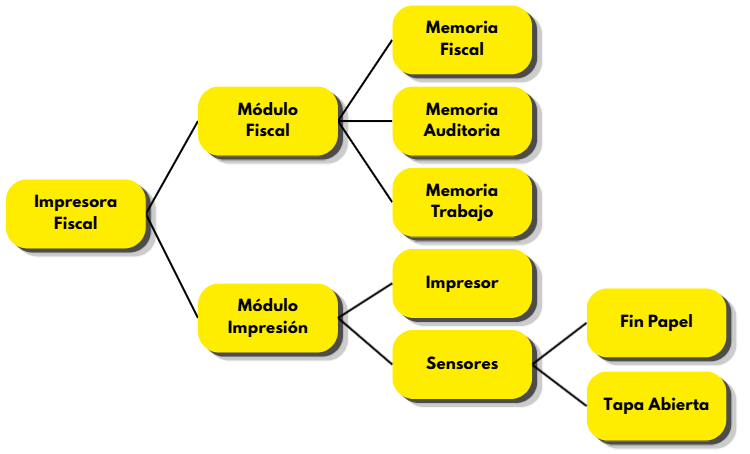
\includegraphics[width=0.9\linewidth]{Img/printer_diagram.png}
    \caption{Estructura de la Impresora Fiscal.}
    \label{fig:imagen2}
\end{figure}

\begin{enumerate}
    \item \textbf{Módulo de Impresión:} Compuesto por el cabezal térmico y sensores de estado (fin de papel, tapa abierta).
    \item \textbf{Módulo fiscal:} El componente más sensible del equipo, encargado de la gestión de tres tipos de memorias independientes:
    \begin{itemize}
        \item \textbf{Memoria Fiscal (MF):} Dispositivo inalterable adherido al chasis que almacena los resúmenes de los Reportes Z, con una cantidad típica de 2000 cierres diarios.
        \item \textbf{Memoria de Auditoría (MA):} Unidad de almacenamiento masivo (generalmente de 2 GB) que guarda copia electrónica fidedigna de cada documento impreso \cite{TheFactoryHKA_Manual_Protocolos}. 
        \item \textbf{Memoria de Trabajo:} Memoria volátil que mantiene los acumuladores de ventas y contadores de la jornada actual, los cuales se transfieren a la MF al ejecutar el cierre diario \cite{TheFactoryHKA_Manual_Protocolos}.
    \end{itemize}
\end{enumerate}

\subsection{Interconexión de Datos: El Rol del Status S1 y SV2}

\par El monitoreo remoto planteado en este trabajo requiere una interconexión física de alto rendimiento para captura de datos en tiempo real. Si bien los sistemas administrativos tradicionales utilizan el estándar serial RS232 para la gestión local \cite{TheFactoryHKA_Manual_Protocolos}, para la integración directa entre el microcontrolador ESP32 y el hardware de la impresora se implementó una \textbf{interfaz de comunicación síncrona}.\\

\par Esta arquitectura de comunicación permite al ESP32 actuar como el controlador principal de la línea, gestionando el flujo de datos mediante señales de sincronismo y control dedicadas. A través de este bus, el firmware realiza el \textit{polling} de información fiscal solicitando tramas específicas como el \textbf{Status S1} (Serial del equipo, RIF y contadores) y \textbf{SV2} (versión de firmware de la impresora) \cite{TheFactoryHKA_Manual_Protocolos, TheFactoryHKA_iSmart_Manual}. La migración no solo garantiza una comunicación de baja latencia y alta confiabilidad, sino que asegura la escalabilidad del sistema ante futuras actualizaciones de hardware, manteniendo la compatibilidad con el dispositivo de transmisión actual de la empresa.

\section{Modelos de Comunicación y Mensajería}

\par En el desarrollo de ecosistemas IIoT, la eficiencia del intercambio de datos depende de la selección de modelos que optimicen el uso del ancho de banda y garantice la integridad de la información. El sistema de transmisión integra tres arquitecturas fundamentales que operan en diferentes niveles de la pila de comunicación, desde la interacción física con el hardware fiscal hasta la visualización en tiempo real en la nube \cite{OASIS_MQTT_v5}.

\subsection{Arquitectura Publicación-Suscripción (Pub/Sub)}

\par A diferencia del modelo tradicional de consulta (request-response), el patrón \textbf{Publicación-Suscripción} desacopla a los productores de datos de los consumidores mediante un intermediario denominado \textit{Broker}, como se muestra en la figura \ref{fig:imagen3} \cite{OASIS_MQTT_v5}. En este proyecto, el microcontrolador ESP32 actúa como publicador de telemetría fiscal, mientras que el Dashboard web se suscribe a tópicos específicos (ej. \texttt{v1/fiscal/serial/json}) para recibir información.\\

\begin{figure} [H]
    \centering
    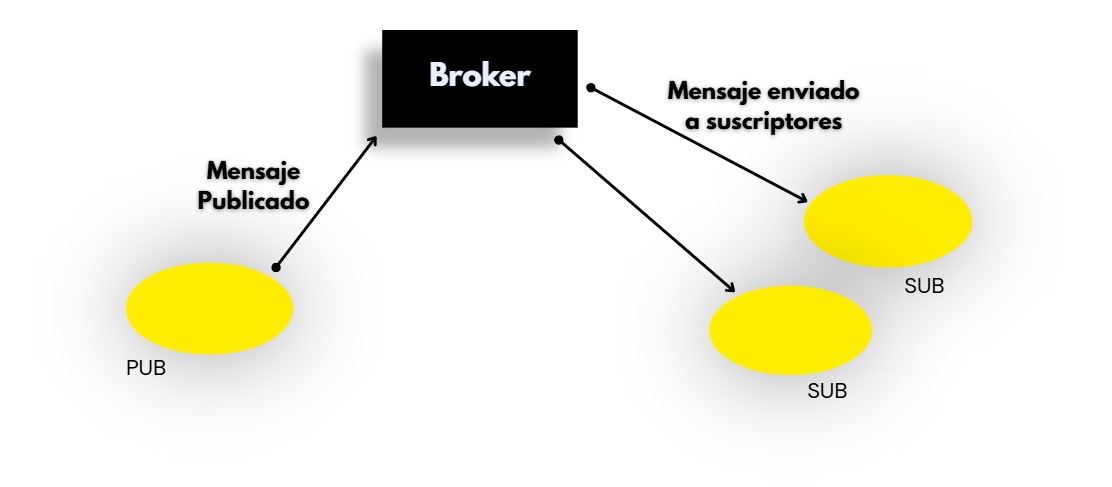
\includegraphics[width=0.95\linewidth]{Img/pubsub_diagram.png}
    \caption{Modelo MQTT de publicación y suscripción.}
    \label{fig:imagen3}
\end{figure}

\par Este modelo ofrece tres dimensiones de desacoplamiento críticas para la robustez industrial \cite{OASIS_MQTT_v5}:

\begin{itemize} 
    \item \textbf{Espacial:} Los dispositivos no necesitan conocer la dirección IP de los demás para comunicarse. 
    \item \textbf{Temporal:} No es necesario que el suscriptor esté en línea al momento de la publicación si se utilizan sesiones persistentes. 
    \item \textbf{Sincronización:} Las operaciones en el ESP32 no se bloquean mientras se envían los datos, permitiendo que la tarea de la impresora continúe su ejecución. 
\end{itemize}

\subsection{Comunicación Bidireccional Full-Duplex (WebSockets)}

\par Para el monitoreo en tiempo real, se implementó el protocolo \textbf{WebSockets}, el cual establece un canal de comunicación persistente y bidireccional sobre una única conexión TCP \cite{RFC6455_WebSockets, Fierro_WebSockets_2017}. A diferencia de HTTP, que requiere una nueva cabecera por cada solicitud, WebSockets reduce drásticamente la latencia mediante un proceso de \textit{handshake} que eleva la conexión de HTTP a un flujo de datos binarios continuo.\\

\par En la arquitectura final de este proyecto, se utiliza \textbf{MQTT sobre WebSockets} \cite{OASIS_MQTT_v5, Fierro_WebSockets_2017}. Esta técnica permite que el Dashboard web encapsule paquetes MQTT dentro de tramas de WebSocket, permitiendo que el navegador \say{hable} directamente con el broker. Esto elimina la necesidad de intermediarios pesados (como Django Channels), simplificando la infraestructura y garantizando que los estados de la impresora se reflejen en pantalla de forma instantanea.

\subsection{Modelo Maestro-Esclavo en Buses Seriales}

\par En el nivel del borde (\textit{Edge}), la interacción entre el microcontrolador y la impresora fiscal se rige por el modelo \textbf{Maestro-Esclavo} \cite{TheFactoryHKA_Manual_Protocolos}. En esta jerarquía, el ESP32 asume el rol de maestro, teniendo el control total sobre el bus de comunicación y decidiendo cuando iniciar la transferencia de datos.\\

\par Para la integración con la impresora HKA80, este modelo se manifiesta a través de un \textbf{bus de comunicación serie síncrono}. El controlador principal genera la \textbf{señal de temporización} y gestiona la \textbf{habilitación del dispositivo periférico} para realizar un  un sondeo \textit{polling} constante de los registros fiscales. Si bien este modelo presenta una alta dependencia del maestro, garantiza un determinismo absoluto en la captura de datos críticos, evitando colisiones en el bus y asegurando que cada trama de \textbf{Status S1} sea recibida y validada antes de proceder con la lógica de red.

\section{Hardware de Alto Rendimiento: ESP32}

\par El núcleo del sistema de transmisión se fundamenta en el ESP32, un sistema en chip (SoC) de bajo consumo diseñado por Espressif Systems que integra conectividad Wi-Fi y Bluetooth de modo dual \cite{Espressif_ESP32_Datasheet}. A diferencia de los microcontroladores convencionales, este dispositivo está diseñado para aplicaciones industriales de IoT, ofreciendo una robustez y versatilidad que permiten manejar simultáneamente tareas de comunicación segura y control de periféricos de alta velocidad (véase la Figura \ref{fig:esp32_physic}).

\begin{figure} [H]
    \centering
    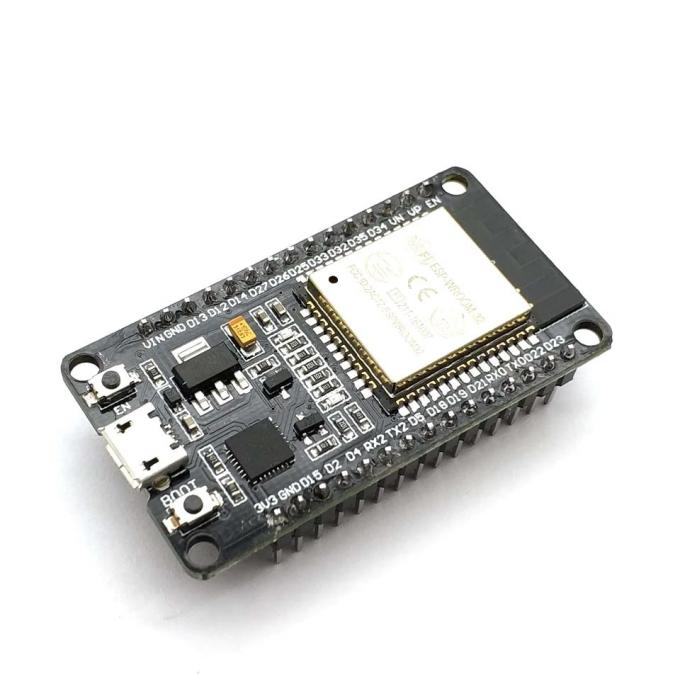
\includegraphics[width=0.5\linewidth]{Img/esp32_physic.png}
    \caption{Vista realista del microcontrolador ESP32.}
    \label{fig:esp32_physic}
\end{figure}

\subsection{Arquitectura de Procesamiento y Multitarea (FreeRTOS)} 

\par El dispositivo integra un microprocesador Xtensa Dual-Core LX6 de 32 bits, capaz de alcanzar un rendimiento de hasta 600 MIPS \cite{Espressif_ESP32_Datasheet}. Esta arquitectura de doble núcleo es un pilar en el proyecto, ya que permite la implementación de un sistema operativo de tiempo real (FreeRTOS) \cite{FreeRTOS_Kernel_Ref}. Mediante la gestión de tareas independientes, el firmware separa la lógica de captura de datos fiscales (tarea de prioridad 5) del stack de comunicación de red, garantizando que el polling de la impresora no se vea interrumpido por las latencias inherentes a la comunicación en la nube.

\subsection{Jerarquía de Memoria y Optimización Crítica} 

\par La gestión de la memoria es el factor determinante para la estabilidad de sistemas que emplean MQTT v5.0 y cifrado TLS/SSL. El ESP32 cuenta físicamente con 520 KB de SRAM interna, la cual se distribuye de forma lógica para optimizar el rendimiento del sistema \cite{Espressif_ESP32_Datasheet}:

\begin{itemize} 
    \item \textbf{IRAM (Instruction RAM):} Espacio de 128 KB reservado para instrucciones críticas y manejadores de interrupciones. El uso eficiente de la IRAM es determinante en sistemas embebidos industriales para alojar stacks de seguridad como Mbed TLS sin comprometer la estabilidad del sistema \cite{Espressif_ESP32_Datasheet}.
    \item \textbf{DRAM (Data RAM):} Utilizada para buffers de datos y el \textit{heap} de la aplicación. Para garantizar la robustez ante fallos de energía, el sistema emplea la \textbf{NVS Flash} (memoria no volátil) para almacenar configuraciones críticas que deben persistir tras un reinicio \cite{Espressif_ESP_IDF_v552}. 
\end{itemize}

\subsection{Seguridad por Hardware y Aceleración Criptográfica}

\par El despliegue de dispositivos IoT en infrestructuras fiscales introduce vulnerabilidades críticas que deben ser mitigadas mediante estándares de crifrado robustos. Sin embargo, la ejecución de algoritmos como AES (Advanced Encryption Standard) o SHA-2 (Secure Hash Algorithm) mediante software consume ciclos de reloj significativos, lo que puede elevar el consumo energético y generar latencia \cite{Espressif_ESP32_Datasheet}.\\

\par El uso de \textbf{Aceleradores Criptográficos por Hardware} en microcontroladores modernos permite delegar estas operaciones matemáticas complejas a módulos de silicio dedicados \cite{Espressif_ESP32_Datasheet, NIST_SP800_52}. Esto garantiza:

\begin{itemize}
    \item \textbf{Integridad de Datos:} Asegura que los registros fiscales no sean alterados durante el tránsito hacia la nube.
    \item \textbf{Autenticación Mutua:} Facilita el intercambio de certificados digitales en el protocolo TLS/SSL de forma eficiente, permitiendo que solo dispositivos autorizados se comuniquen con el servidor central \cite{RFC5246_TLS12}. 
\end{itemize}

\subsection{Interfaces de Comunicación y Capacidad Sensorial} 

\par El sistema de transmisión aprovecha la matriz de periféricos avanzados del chip para la integración con el ecosistema fiscal \cite{Espressif_ESP32_Datasheet}. Se utiliza una interfaz de comunicación física operando a una frecuencia optimizada, lo que asegura un intercanbio de datos constante y de baja latencia con hardware de impresión. Esta interfaz permite al ESP32 actuar como el maestro de la comunicación, gestionando líneas dedicadas para la captura inmediata de registros de estado.\\

\par Asimismo, la radio integrada de 2.4 GHz permite la interconexión bajo los estándares 802.11 b/g/n, posicionando al dispositivo como un Gateway industrial que cumple con las capas de detección e intercambio de datos descritas en la arquitectura IoT industrial \cite{Espressif_ESP32_Datasheet}.

\section{Desarrollo Profesional con ESP-IDF y FreeRTOS}

\par A diferencia de los entornos de prototipado rápido, la implementación de un sistema de monitoreo fiscal industrial exige un control granular sobre los recursos del hardware y una ejecución determinista de las tareas. Por ello, este proyecto se fundamenta en el \textbf{Espressif IoT Development Framework (ESP-IDF)}, el entorno de desarrollo nativo que permite explotar la arquitectura de doble núcleo del ESP32 mediante el uso de un \textbf{Sistema Operativo de Tiempo Real (FreeRTOS)} \cite{Espressif_ESP_IDF_v552, FreeRTOS_Kernel_Ref}.

\subsection{Gestión de Tareas y Sincronización (Mutexes y Colas)}

\par En entornos industriales, el monitoreo de equipos fiscales exige una ejecución determinística. El uso de un RTOS (Real-Time Operating System) como FreeRTOS permite la abstracción del hardware mediante la implementación de un planificador de tareas (\textit{Scheduler}) basado en prioridades \cite{FreeRTOS_Kernel_Ref}. Esta arquitectura es fundamental para garantizar que los procesos de comunicación no bloqueen la lectura crítica de datos fiscales.\\

\par La robustez del firmware se fundamenta en tres pilares conceptuales de la computación concurrente haciendo que las tareas se fragmenten tal como muestra la figura \ref{fig:imagen4}:

\begin{figure} [H]
    \centering
    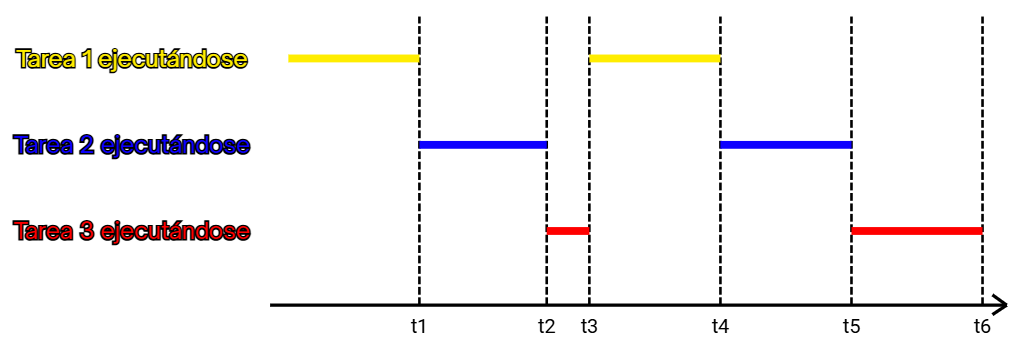
\includegraphics[width=0.9\linewidth]{Img/scheuler_diagram.png}
    \caption{Diagrama de ejecución de tres tareas en distintos instantes de tiempo.}
    \label{fig:imagen4}
\end{figure}

\begin{itemize}
    \item \textbf{Planificación por Prioridades (Preemptive Scheduling):} Permite que el procesador alterne entre múltiples hilos de ejecución. En sistema IoT, esto asegura que las tareas de alta prioridad, como el procesamiento de tramas de comunicación como la impresora, se ejecuten imediantamente, mientras que las tareas de menor prioridad, como el envío de telemetría, se procesen en los tiempos de espera del CPU \cite{FreeRTOS_Kernel_Ref}.
    \item \textbf{Mecanismos de Exclusión Mutua (Mutex):} El acceso concurrente a recursos compartidos, como los buses de comunicación, representa un riesgo de corrupción de datos. El uso de \textit{Mutexes} garantiza que solo una tarea posea el control del recurso en un momento dado, evitando condiciones de carrera (\textit{race conditions}) que podrían comprometer la integridad de la información tributaria \cite{FreeRTOS_Kernel_Ref}.
    \item \textbf{Sincronización mediante Semáforos y Colas (Queues):} Estos mecanismos permiten la comunicación inter-tareas. Las colas de mensajes facilitan el paso de datos entre el núcleo que gestiona la lógica de la impresora y el núcleo encargado de la pila de red, permitiendo una arquitectura desacoplada y escalable \cite{FreeRTOS_Kernel_Ref}.
\end{itemize}

\section{Protocolos de Red y Transporte}

\par La arquitectura de comunicaciones del sistema de transmisión se fundamenta en una pila de protocolos diseñados para entornos de alta confiabilidad y recursos restringidos. La integración del estándar \textbf{MQTT v5.0} sobre capas de seguridad \textbf{TLS/SSL}, sumada a la eficiencia del bus para la comunicación local, constituye una infraestructura robusta que garantiza la integridad de la información fiscal desde el borde hasta la nube \cite{OASIS_MQTT_v5, RFC5246_TLS12}.

\subsection{MQTT v5.0: Características Avanzadas y Trazabilidad}

\par El protocolo \textbf{MQTT (Message Queuning Telemetry Transport)} es un estándar de mensajería basado en el modelo publicación-suscripción, optimizado para redes de baja tasa de bits y alta latencia \cite{OASIS_MQTT_v5}. Para este proyecto, se implementó la versión \textbf{5.0}, la cual representa una evolución crítica respecto a su predecesor (v3.1.1), introduciendo características de escalabilidad y reporte de errores superiores.\\

\par Una de las herramientas integradas en el firmware es el uso de las \textbf{User Properties}. Estas permiten adjuntar metadatos personalizados en formato clave-valor a las tramas de publicación (PUBLISH), facilitando una \textbf{trazabilidad transparente} en sistemas complejos. En el sistema de transmisi\'on, estas propiedades se utilizan para enviar información de autodiagnóstico y modelo de hardware sin sobrecargar el \textit{payload} JSON del mensaje. Además, el uso de \textbf{Reason Codes} en todos los paquetes de reconocimiento (ACKs) permite que el ESP32 reciba una retoralimentación detallada del broker ante cualquier fallo de comunicación, mejorando la resilencia operativa del nodo sensor \cite{OASIS_MQTT_v5}.

\subsection{Seguridad en la Capa de Transporte (TLS/SSL)}

\par Dado que el sistema maneja información tributaria sensible, la seguridad es un requisito de diseño mandatorio. El sistema utiliza el protocolo \textbf{Transport Layer Security (TLS)}, su sucesor del Secure Socket Layer (SSL), para proporcionar un canal cifrado sobre TCP que garantiza la \textbf{confidencialidad, integridad, y autenticidad} de los datos \cite{RFC5246_TLS12, NIST_SP800_52}.\\

\par La implementación se basa en un proceso de \textbf{Handshake} mediante el cual el ESP32 y el broker negocian parámetros criptográficos y validan identidades a través de certificados digitales. Siguiendo las recomendaciones internacionales, el sistema opera sobre el \textbf{puerto seguro 8883} (IANA: \textit{secure-mqtt}), lo que mitiga riesgos criticos como el espionaje pasivo (\textit{eavesdropping}) y la inyección de contenido malicioso \cite{NIST_SP800_52}. Esta capa de seguridad asegura que, incluso si las tramas son interceptadas en la red pública, la información permanezca ininteligible para atacantes externos.

\subsection{Comunicación Serial e Interfaz de Datos Local}

\par En el nivel de borde, la captura de datos fiscales se realiza a través una \textbf{interfaz de comunicación síncrona de alto rendimiento} \cite{TheFactoryHKA_Manual_Protocolos}. A diferencia de las interfaces seriales asíncronas tradicionales (UART), este método permite el intercambio de información en modo \textit{full-duplex} con un determinismo superior.\\

\par El sistema de transmisi\'on opera bajo una jerarquía de \textbf{Maestro-Esclavo}, donde el microcontrolador ESP32 actúa como el nodo maestro que genera la señal de \textbf{sincronización (o temporización)} y gestiona la línea de \textbf{habilitación del periférico} para orquestar la comunicación con la impresora fiscal. Esta arquitectura garantiza un determinismo absoluto en la captura de registros críticos (Status S1/SV2), ya que el uso de \textbf{vías de transmisión y recepción independientes} evita colisiones de datos y permiten velocidades de transferencia significativamente superiores a las de una conexión RS232 convenicional \cite{TheFactoryHKA_Manual_Protocolos}. El uso de este bus síncrono es lo que permite que el sistema mantenga una frecuencia de muestreo constante de 5 segundos sin interferir con las operaciones internas del firmware de la impresora.

\section{Estructuraci\'on de Datos con JSON}

\par En la arquitectura de comunicaciones de este proyecto, la representac\'on y el empaquetado de la informaci\'on fiscal se fundamentan en el formato \textbf{JSON (JavaScript Object Notation)}. Este es un est\'andar de intercambio de datos ligero, basado en una estructura de pares clave-valor, que permite una legibilidad superior tanto para humanos como para m\'aquinas \cite{Salazar_IoT_2014}. Su adopción en sistemas IIoT es cr\'itica debido a su independencia de lenguaje, lo que facilita la interoperabilidad entre el firmware desarrollado en \textbf{C (ESP-IDF)}, el broker MQTT y el backend en \textbf{Python (Django)}.\\

\par A diferencia de otros lenguajes del mercado como XML, JSON ofrece una sobrecarga (\textit{overhead}) significativamente menor, lo que se traduce en paquetes m\'as pequeños y un menor consumo de energ\'ia y memoria en el microcontrolador \cite{Salazar_IoT_2014}. En el sistema de transmisi\'on, los paquetes JSON se encapsulan tanto en tramas MQTT como en sobres de WebSockets para su transporte hacia la nube.

\section{Integración Web y Monitoreo en Tiempo Real}

\par La capa de visualizaci\'on del sistema de transmisi\'on trasciende los portales web est\'aticos mediante la implementaci\'on de tecnolog\'ias de flujo de datos continuo. El uso de protocolos de baja latencia garantiza que los estados de la impresora fiscal se reflejen en el Dashboard con un retraso imperceptible, cumpliendo con los est\'andares de monitoreo industrial en tiempo real \cite{RFC6455_WebSockets}.

\subsection{Protocolo WebSockets}

\par El protocolo \textbf{WebSocket}, definido en el RFC 6455, proporciona canales de comunicaci\'on \textbf{full-duplex} sobre una \'unica conexi\'on TCP \cite{RFC6455_WebSockets}. A diferencia del protocolo HTTP, que es de naturaleza \textit{half-duplex} y carece de estado, WebSocket permite que el servidor env\'ie informaci\'on al cliente de forma proactiva sin esperar una solicitud previa.\\

\par El establecimiento de la comunicaci\'on se rige por el proceso \textbf{Handshake}, el cual inicia como una solicitud HTTP convencional. Durante este intercambio, el cliente y el servidor acuerdan una \say{actualizaci\'on de protocolo} (\textit{Protocol Upgrade}), transformando la conexi\'on HTTP en un flujo de datos binarios bidireccional y persistente. Una vez establecida, se eliminan la cabeceras (\textit{headers}) repetitivas de HTTP, lo que reduce dr\'asticamente el payload de la conexi\'on y permite una transferencia de datos m\'as eficiente y con menor latencia en comparaci\'on con t\'ecnicas como el \textit{long polling} \cite{Fierro_WebSockets_2017}.

\subsection{MQTT sobre WebSockets}

\par En la arquitectura final de este proyecto, se implement\'o la t\'ecnica de \textbf{t\'unel o encapsulamiento de MQTT sobre WebSockets}. Esta integraci\'on es fundamental debido a que los navegadores web actuales no permiten la apertura de conexione TCP crudas (\textit{raw sockets}) necesarias para el protocolo MQTT nativo \cite{OASIS_MQTT_v5, Fierro_WebSockets_2017}.\\

\par Bajo este esquema, la conexi\'on WebSocket act\'ua como una tuber\'ia externa o \say{sobre} para los paquetes MQTT. El broker HiveMQ coloca cada paquete MQTT (como CONNECT o PUBLISH) dentro de una trama binaria de WebSocket para enviarla al Dashboard, donde la librer\'ia de cliente JavaScript (Paho) desaempaqueta la informaci\'on y la procesa como una trama de red est\'andar \cite{OASIS_MQTT_v5}. En el sistema de transmisi\'on, esta comunicaci\'on segura se orquesta a trav\'es del \textbf{puerto 8000}, lo que permite atravesar firewalls corporativos que habitualmente bloquean los puertos est\'andar de MQTT (1883/8883) pero permiten el tr\'afico web convencional. Esta arquitectura desacoplada garantiza la \textbf{resilencia cibern\'etica} del sistema, permitiendo un monitoreo directo entre el navegador y el broker sin intermediarios adicionales.

\section{Arquitectura de Gesti\'on y Orquestaci\'on: Framework Django}

\par La capa superior del ecosistema de transmici\'on requiere de un motor robusto capaz de centralizar la informaci\'on, gestionar la seguridad de acceso y servir de puente entre el almacenamiento de datos y la interfaz de usuario. Para este prop\'osito, se seleccion\'o \textbf{Django}, un framework web de alto nivel basado en el lenguaje de programaci\'on \textbf{Python} \cite{Django_v5_Doc}. Python se caracteriza por ser un lenguaje interpretado de prop\'osito general, cuya filosof\'ia hace hincap\'ie en la legibilidad del c\'odigo y la eficiencia t\'ecnica, caracter\'isticas esenciales para el mantenimiento de sistemas industriales a largo plazo.

\subsection{Patr\'on de Diseño MVT (Model-View-Template)}

\par Django fundamenta su operaci\'on en una arquitectura denominada \textbf{Model-View-Template}, la cual permite una separaci\'on clara de responsabilidades en el servidor de aplicaciones \cite{Django_v5_Doc}:

\begin{itemize}
    \item \textbf{Modelo (Model):} Representa la fuente de informaci\'on definitiva de los datos. En este proyecto, el modelo define la estructura de las tablas donde se gestionan los equipos fiscales y los registros de auditor\'ia.
    \item \textbf{Vista (View):} Act\'ua como el mediador l\'ogico que procesa las solicitudes de los usuarios y retorna las respuestas adecuadas. Es el componente encargado de la orquestaci\'on del sistema.
    \item \textbf{Plantilla (Template):} Es la capa de presentaci\'on que define c\'omo se muestran los datos al usuario final, integrando el contenido generado por el servidor con el Dashboard web.
\end{itemize}

\subsection{Arquitectura Web Eficiente: HTMX y la comunicación Asíncrona}

\par En la evolución del desarrollo web para sistemas embebidos, ha surgido una dicotomía entre las aplicaciones tradicionales multipágina (MPA) y las aplicaciones de una sola página (SPA) basadas en pesados \textit{frameworks} de JavaScript. HTMX se presenta como una alternativa que permite extender las capacidades del HTML para realizar peticiones AJAX, WebSockets y Server-Sent Events directamente desde los atributos del mercado \cite{HTMX_Doc}.\\

\par La relevancia de HTMX en este proyecto radica en:

\begin{itemize}
    \item \textbf{Reducción de la Carga en el Cliente:} Al procesar la lógica de presentación en el servidor (Django) y enviar solo fragmentos de HTML al navegador, se minimiza la necesidad de procesar grandes archivos de \textit{scripts} en el dispositivo del usuario final.
    \item \textbf{Reactividad sin Complejidad:} Permite actualizaciones parciales del Dashboard web (como el estado de conexión de la impresora) en tiempo real, manteniendo la simplicidad del protocolo HTTP sin la sobrecarga de un motor de renderizado del lado del cliente.
\end{itemize}

\subsection{Gesti\'on Administrativa y Persistencia}

\par Una de las caracter\'isticas de este framework es su capacidad de generar din\'amicamente una \textbf{interfaz administrativa} (Admin Panel). Esta herramienta permite que los administradores del sistema en \textbf{The Factory HKA} realicen operaciones \textbf{CRUD} (Crear, Leer, Actualizar y Borrar) sobre la base de datos de los equipos de forma segura, sin necesidad de interactuar directamente con el motor de base de datos SQL \cite{Django_v5_Doc}.\\

\par En la arquitectura del dispositivo de transmisión, Django cumple el rol de Servidor de Aplicaciones, diferenci\'andose de un servidor web est\'atico al procesar l\'ogica compleja y garantizar que solo usuarios autenticados puedan acceder al monitoreo en tiempo real de los registros fiscales. Esta robustez, sumada a su enfoque en la reutilizaci\'on de componentes y el principio \textit{don't repeat yourself} (DRY), asegura que el sistema sea escalable ante el crecimiento del parque de impresoras instaladas \cite{Django_v5_Doc}.